\documentclass[a4paper]{article}
\usepackage[utf8]{inputenc}
\usepackage[spanish, es-tabla, es-noshorthands]{babel}
\usepackage[table,xcdraw]{xcolor}
\usepackage[a4paper, footnotesep = 1cm, width=22cm, top=2.5cm, height=25cm, textwidth=20cm, textheight=25cm]{geometry}
%\geometry{showframe}

\usepackage{tikz}
\usepackage{amsmath}
\usepackage{amsfonts}
\usepackage{amssymb}
\usepackage{float}
\usepackage{graphicx}
\usepackage{caption}
\usepackage{subcaption}
\usepackage{multicol}
\usepackage{multirow}
\usepackage{wrapfig}
\setlength{\doublerulesep}{\arrayrulewidth}
\usepackage{booktabs}

\usepackage{hyperref}
\hypersetup{
    colorlinks=true,
    linkcolor=blue,
    filecolor=magenta,      
    urlcolor=blue,
    citecolor=blue,    
}

\newcommand{\note}[1]{
	\begin{center}
		\huge{ \textcolor{red}{#1} }
	\end{center}
}

\setcounter{topnumber}{2}
\setcounter{bottomnumber}{2}
\setcounter{totalnumber}{4}
\renewcommand{\topfraction}{0.85}
\renewcommand{\bottomfraction}{0.85}
\renewcommand{\textfraction}{0.15}
\renewcommand{\floatpagefraction}{0.8}
\renewcommand{\textfraction}{0.1}
\setlength{\floatsep}{5pt plus 2pt minus 2pt}
\setlength{\textfloatsep}{5pt plus 2pt minus 2pt}
\setlength{\intextsep}{5pt plus 2pt minus 2pt}

\newcommand{\quotes}[1]{``#1''}
\usepackage{array}
\newcolumntype{C}[1]{>{\centering\let\newline\\\arraybackslash\hspace{0pt}}m{#1}}
\usepackage[american]{circuitikz}
\usetikzlibrary{calc}
\usepackage{fancyhdr}
\usepackage{units} 

\graphicspath{{../Ejercicio-1/}{../Ejercicio-2/}{../Ejercicio-3/}{../Ejercicio-4/}{../ParteI/}{../ParteII/}{../ParteIII/}{../ParteIV/}}

\pagestyle{fancy}
\fancyhf{}
\lhead{22.14 - Electrónica IV}
\rhead{Mechoulam, Lambertucci, Londero}
\rfoot{Página \thepage}


\begin{document}

\subsection{Introducción}

Dada una fuente Boost con una tensión de entrada $12 \ V$ y frecuencia de switching de $60 \ kHz$, se buscó determinar el Duty Cicle necesario tal que la tensión de salida sea de $24 \ V$ y tenga una variación del $5\%$. Cabe notar que esta fuente Boost es una no ideal ya que se considera la resistencia de la bobina $R_4 = 2 \ \Omega$.

\begin{figure}[H]
	\centering
	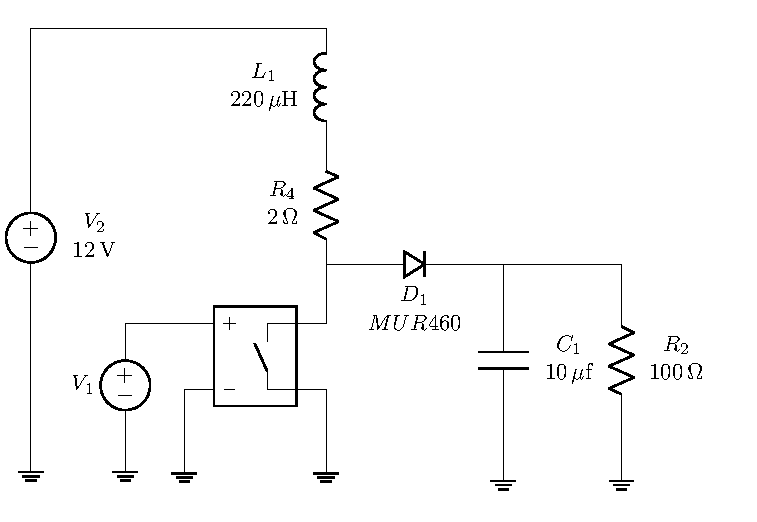
\includegraphics[width=0.7\linewidth, page=1]{ImagenesEjercicio-2/CircuitsEj2}
	\caption{Circuito de fuente Boost con llave ideal.}
	\label{fig:ej2:circuito}
\end{figure}

\subsection{Calculo del Duty Cicle}

Para el período de encendido, el hemicircuito es el siguiente. 

\begin{figure}[H]
	\centering
	\includegraphics[width=0.8\linewidth, page=2]{ImagenesEjercicio-2/CircuitsEj2}
	\caption{Circuito de fuente Boost con llave cerrada.}
	\label{fig:ej2:off}
\end{figure}

Planteando las mallas 1 y 2 se obtienen las siguientes ecuaciones:
\begin{equation*}
\begin{cases}
V_2 - L \dot{I_L} - R_4 I_L = 0 \\
C \dot{V_C} = -\frac{V_O}{R_2}
\end{cases}
\end{equation*}

Operando algebraicamente se obtienen las matrices: 
\begin{equation}
\mathbb{A}_{on} =  \begin{pmatrix}
	-R_4/L & 0 \\
	0 & -1/ C R_2
\end{pmatrix} \ \ \
\mathbb{B}_{on} =  \begin{pmatrix}
	1/L \\
	0
\end{pmatrix} \ \ \
\mathbb{C}_{on} =  \begin{pmatrix}
	0 & 1 \\
\end{pmatrix}
\end{equation}

Por otro lado, durante el apagado, el hemicircuito resultante es el que se muestra a continuación.

\begin{figure}[H]
	\centering
	\includegraphics[width=0.8\linewidth, page=3]{ImagenesEjercicio-2/CircuitsEj2}
	\caption{Circuito de fuente Boost con llave cerrada.}
	\label{fig:ej2:on}
\end{figure}

De forma similar al caso anterior, planteando la malla externa y la suma de corrientes en el nodo $A$, se obtienen las ecuaciones siguientes:

\begin{equation*}
\begin{cases}
V_2 - L \dot{I_L} - R_4 I_L - V_O = 0 \\
I_L = I_C + I_O = C\dot{V_C} + \frac{V_O}{R_2}
\end{cases}
\end{equation*}

Operando algebraicamente se obtienen las matrices: 
\begin{equation}
\mathbb{A}_{off} =  \begin{pmatrix}
	-R_4/L & -1/L \\
	1/C & -1/ C R_2
\end{pmatrix} \ \ \
\mathbb{B}_{off} =  \begin{pmatrix}
	1/L \\
	0
\end{pmatrix} \ \ \
\mathbb{C}_{off} =  \begin{pmatrix}
	0 & 1 \\
\end{pmatrix}
\end{equation}

Se definen las matrices $\mathbb{A}$, $\mathbb{B}$ y $\mathbb{C}$ de la forma:
\begin{equation}
\mathbb{A} = \mathbb{A}_{on} \cdot d + \mathbb{A}_{off} \cdot (1-d) =  \begin{pmatrix}
	-R_4/L & (d-1)/L \\
	(1-d)/C & -1/ C R_2
\end{pmatrix}
\end{equation}

\begin{equation}
\mathbb{B} = \mathbb{B}_{on} \cdot d + \mathbb{B}_{off} \cdot (1-d) = \begin{pmatrix}
	1/L \\
	0
\end{pmatrix}
\end{equation}

\begin{equation}
\mathbb{C} = \mathbb{C}_{on} \cdot d + \mathbb{C}_{off} \cdot (1-d) = \begin{pmatrix}
	0 & 1
\end{pmatrix}
\end{equation}

Finalmente, dado que la transferencia en el permanente esta dada por $H = -\mathbb{C} \cdot \mathbb{A}^{-1} \cdot \mathbb{B}$, se obtiene que:
\begin{equation}
H = \frac{\left( 1 - d \right) R_2}{R_2 d^2 - 2 R_2 d + R_2 + R_4}
\end{equation}

Reemplazando con $R_4 = 2 \ \Omega$, $R_2 = 100 \ \Omega$, y sabiendo que se busca que $H = V_o / V_2 = 2$, se obtiene que el Duty Cicle puede tomar 2 valores posibles: $d = 0.544$ y $d = 0.956$. Como se sabe que las fuentes switching pierden linelaidad al tomar valores de Duty Cicle elevados, se descarta el segundo valor hallado.

Por otro lado, utilizando la transferencia de la fuente Boost ideal, es decir sin $R_4$, se puede obtener el Duty Cicle deseado:
\begin{align*}
V_o &= \frac{V_2}{1 - d}	\\
1 - d &= \frac{V_2}{V_o} = \frac{12 \ V}{24 \ V} \\
d &= 0.5
\end{align*}

Este valor es cercano al obtenido considerando la alinealidad.
\note{TIENE SENTIDO??}

\end{document}